\documentclass[12pt]{article}
\usepackage{fancyhdr}
\usepackage{float}
\usepackage{amsmath}
\usepackage{graphicx}
\usepackage{listings}
\lstset{language=C++,literate={\ \ }{{\ }}1}
\usepackage{hyperref}
\title{MIDI file player}
%TODO:change the date
\date{01/02/2016}
\author{Davide Botti,Cristiano Di Marco}

\begin{document}
\maketitle
\pagenumbering{gobble}
\pagestyle{fancy}
\fancyhead{}
\fancyfoot{}
\fancyfoot[R]{\thepage}
\newpage
\pagenumbering{arabic}
\tableofcontents

\newpage
\section{Introduction} \label{sec:intro}
 The aim of this project is to implement a simple MIDI file player inside the board STM32f4 discovery. In fact the board is equipped with a common DAC by which the music can be reproduced, a 192KB RAM memory,1MB flash memory (non-volatile memory), in which we loaded the code and other useful files (more details in next sections) and with an ARM Cortex M4 processor; so it's a quite powerful board. We use the operating system \href{https://miosix.org/}{Miosix} as it provides functionalities such as primitives to read/write to the serial line, and to send data to the DAC peripheral.\newline
 \begin{figure}[H]
 	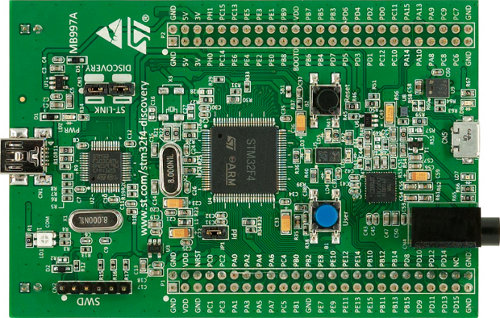
\includegraphics[width=0.8\textwidth]{STM32F4-Discovery-Board.jpg}
 	\caption{STM32f4}
 	\label{fig:STM32f4Discovery}
 \end{figure}
In order to implement what is written further, you need a board, a program to send binaries into the board (like STLink), and a patched C compiler in order to compile for the ARM Cortex M4 (more details in the \ref{sec:used}th section).

\section{MIDI structure} \label{sec:structure}
One important thing (actually the most important) in order to implement a MIDI player, was to understand the basic structure of a MIDI file: the file indeed has a fixed structure that divides it in three subsections: 
\begin{description} 
	\item[header section] The header chunk consists of a literal string denoting the header, a length indicator, the format of the MIDI file, the number of tracks in the file, and a timing value specifying delta time units. This is an introductory section, so apart from the information about the time, can be skipped by our program.
	\item[body section] the body section consists of a series of MIDI events, such as the reproduction of a note, a pause, a change in time or a change of the instrument (so called meta-events). Actually this is the most important part, because here we can find all the notes that create the music.
	\item[end section] this section simply indicates the end of the MIDI file, and is always composed of 4 bytes: \emph{00 FF 2F 00}.
\end{description}
As you can easily understand, the most important section is the body, where we can actually find the notes that we're going to play. In practice, a MIDI file is a sequence of "MIDI messages" that represent the real music.\newline 
There are two broad message categories: 
\begin{description} 
	\item[system message] system messages are non-MIDI data of various sorts consisting of a fixed prefix, type indicator, a length field, and actual event data. For example, this messages indicate what type of instrument is playing, or a change in the rhythm.
	\item[channel message] consist of a delta time since the last message, and three bytes that can vary according to the specific type of message. For example, these bytes can represent the reproduction of a note, a pause, a control change ect...
\end{description}
In our project we focus our attention on channel-messages, that represent the real music, in particular on the \textbf{event 9x}, that indicates the reproduction of a note.

\subsection{MIDI messages}
Here we would like to underline some MIDI messages and explain a bit their structure.Because of the great heterogeneity of MIDI message types, we had to make some assumptions and analyze only a subset of these. Every message is composed of three bytes, that indicates respectively the event type, the note and the velocity. In particular, the note is simply a number that encodes the information of the pitch (for example, a C2 is the number 48,C3 is number 60 and so on..). 
Every message is preceded by a timestamp that indicates the delta time from the previous event.\newline
Eventually, a complete channel-message is composed of: \newline
\emph{delta-time,event-id,note-number,velocity} \newline
Here we provide some more details about these fields:\newline
\begin{description}
	\item[delta-time] it is the relative time from the current time and indicates when the message starts. We have to take particular attention to this field because it has variable length: in particular, if the first byte cannot represent the time (because it is too short), the MIDI standard adds another byte to the first, and so on if also the second byte cannot represent the time interval.
	\item[message-id] type of message; as already mentioned, an event-id of value 9x represents the reproduction of a note, instead message 8x the stop of a note.
	\item[note-number] the pitch of the note: these numbers starts from 0 (C-2) and linearly increase until 127 (G8). In this way,every note is uniquely identified by a number; this makes easy the recognition of the note.
	\item[velocity] a measure of how rapidly and forcefully a key on a keyboard is pressed.
\end{description}
Here we report the messages which we should take care of; the useful messages are only two: the messages that indicates the reproduction of the note, and the messages that indicates the pause of a note.
\begin{description} 
	\item[event 9x]  as already mentioned, this message represents the reproduction of a note, or a pause if the velocity is equal to zero. The latter 4 bits represents the channel of the note.
	\item[event 8x] this message represents instead the end of a note. The latter 4 bits represents the channel of the note.
\end{description}

%TODO: check the code before deadline
\section{Algorithm} \label{sec:algorithm}
The algorithm (all written in C++) implements a simple parser:there is a main thread that reads from the serial port each byte and sets the note to be played. Another thread takes care of playing the current note (previously set by the main thread).In practice, this is a producer-consumer pattern in which the producer reads bytes from the serial port and the consumer continuously play notes, reading from a one-byte buffer.

\subsection{Preliminary steps}
First we have to understand how to transfer bytes: we send it via the serial port of the board, but this requires some preliminary steps, in particular:
\begin{itemize}
	\item open a MIDI port (this passage seems to be done only on Windows).
	\item open the MIDI file with a program that allows you to send it via a specific port; not all the programs allow this, for example by \textit{MidiOx}  you can send it via different output ports.
	\item connect the MIDI port to the serial port:we did this by \textit{hairless-MIDI-serial},a simple software that allows to send a data stream over the serial port.
	\item sample some notes and convert it in order to have a C-style header file which contains a kind of waveform of the notes.
\end{itemize}
Following the previous steps, we managed to transfer the bytes through the serial line and to obtain different header files, that contain an array of bytes that represents the waveform of a note. Now we are ready to play music thanks to our algorithm.

\subsection{Reading from the serial}
The main thread reads from the serial port and waits for an event 0x9x (it is a kind of a parser). When it finds that specific byte, reads the note, the velocity of the next event, stores this information in a buffer and waits the player to finish the reproduction. The producer algorithm is reported below:

\begin{lstlisting}
//Producer code.
\end{lstlisting}

The function parse\_byte is called from the main function and takes as input a single byte: if this byte is 0x90 (or 91,92..,9F), the program fetch the pitch, the velocity of the next event and locks the mutex in order to set the current note to be played. Please note that the algorithm does not care about the channel of the note: in fact the following line:
\begin{lstlisting}
	if((c & 0b10010000)==0x90)
\end{lstlisting}
masks the byte in order to discard the latter 4 bits.\newline
Finally, the main thread set the shared variable current\_note and unlocks the mutex so the consumer can access it.

\subsection{Playing notes}
This is the core of the project.In order to play notes, knowing the pitch of the note, we stored in the flash memory of the board header files that correspond to sampled notes produced with Audacity.These header files are produced by a program, \textit{convert.exe}, that takes as input a .Wav file and returns a .h header C-style file, that contains the bytes of the notes.Then, we pass the array contained into these headers to a costructor that creates a custom object (\textit{ADPCMSound}, can be found in Miosix).This object represents the "sound" to be played.\newline
 When the producer signals the consumer that a new note is ready, the player checks which note it has to play (by a simple switch() statement) and sends the corresponding bytes to the output DAC. Here is the code of our player:

\begin{lstlisting}
// consumer code
\end{lstlisting}
%TODO: fix this part, bad written
The player continuously plays notes, reading from the shared buffer in a secure manner (thanks to the mutex). The consumer does not wait for the producer to store another note in the buffer, but plays indefinitely the current note: in this way the MIDI file can be reproduced with the right speed, because the notes arrive at a certain instant in time, and if our threads wait each other, this will bring to a time degradation.\newline
In order to pass the bytes to the peripheral, our player uses a custom Miosix class, \textit{Player}, that manages the transmission between our program and the DAC peripheral.

\subsection{Known issues}
Here we report some issues that are present in our program; this issues are mainly due to the academic purpose of the project. That is, our goal was not to implement a real MIDI player but only to deal with problems studied only theoretically (such as producer-consumer pattern).
\begin{description}
	\item[File format] Our MIDI player can parse only a subset of MIDI files in which the reproduction of a note is "clearly" specified. There are in fact cases in which, for optimization reasons, the notes are queued after a single event 90. If that happen, our parser will fail in recognizing that notes and will not play them.
	\item[time] The MIDI player does not manage the speed of the song, but it plays it with a standard and unchangeable speed.
	%TODO:change it if we manage or not the duration of the notes
	\item[note duration] Our MIDI player reproduces only semiminime, crome and semicrome.
	\item[instrument type] The player does not recognize the playing instrument: so all the notes have the same timbro (this can be easily fixed by checking the channel of the note, instead of masking it).
	%TODO:maybe can be deleted
	\item[note size] The board has a 1MB flash memory that could saturate if we upload too much notes; this could be a problem if we need to reproduce a complex melody with a lot of notes.
\end{description}

\subsection{About the code}

The entire code can be found in our github repository: \url{https://github.com/dade92/es_project}

\section{Used Software} \label{sec:used}
\begin{description} 
	\item[Miosix-kernel] Kernel; can be found at \url{https://miosix.org/}
	\item[gcc patch] patch for the gcc compiler; more info at \url{https://miosix.org/wiki/index.php?title=Miosix_Toolchain}
	\item[Dev-c++] to write c++  code.
	\item[loop-midi] to open a MIDI port (necessary only on Windows). Can be found at \url{http://www.tobias-erichsen.de/software/loopmidi.html}
	\item[midi-ox] to reproduce the MIDI and send it to the MIDI port. Can be found at \url{http://www.midiox.com/}
	\item[hairless-midiserial] to interface the MIDI port with the serial port. Can be found at \url{http://projectgus.github.io/hairless-midiserial/}
	\item[QSTlink2] to program the board.
	\item[Audcacity] to produce the notes.
	\item[convert.exe] c++ written program to convert the .Wav files  of the notes into .h header files.
	\item[program to generate MIDI] used to generate MIDI files.
	\item[Hex editor] to read the MIDI file in a hexadecimal manner.
\end{description}

\end{document}